\section{CNN Architecture}
\begin{frame}{}
    \LARGE CNN: \textbf{Architecture}
\end{frame}

\begin{frame}{CNN Architecture}
    \textbf{What makes a Convolutional Neural Network?}
    
    Characterised by “Convolutional Layer” – they are able to detect “abstract features” and “almost ideas within the image”

    \newline

    \begin{figure}
    \centering
    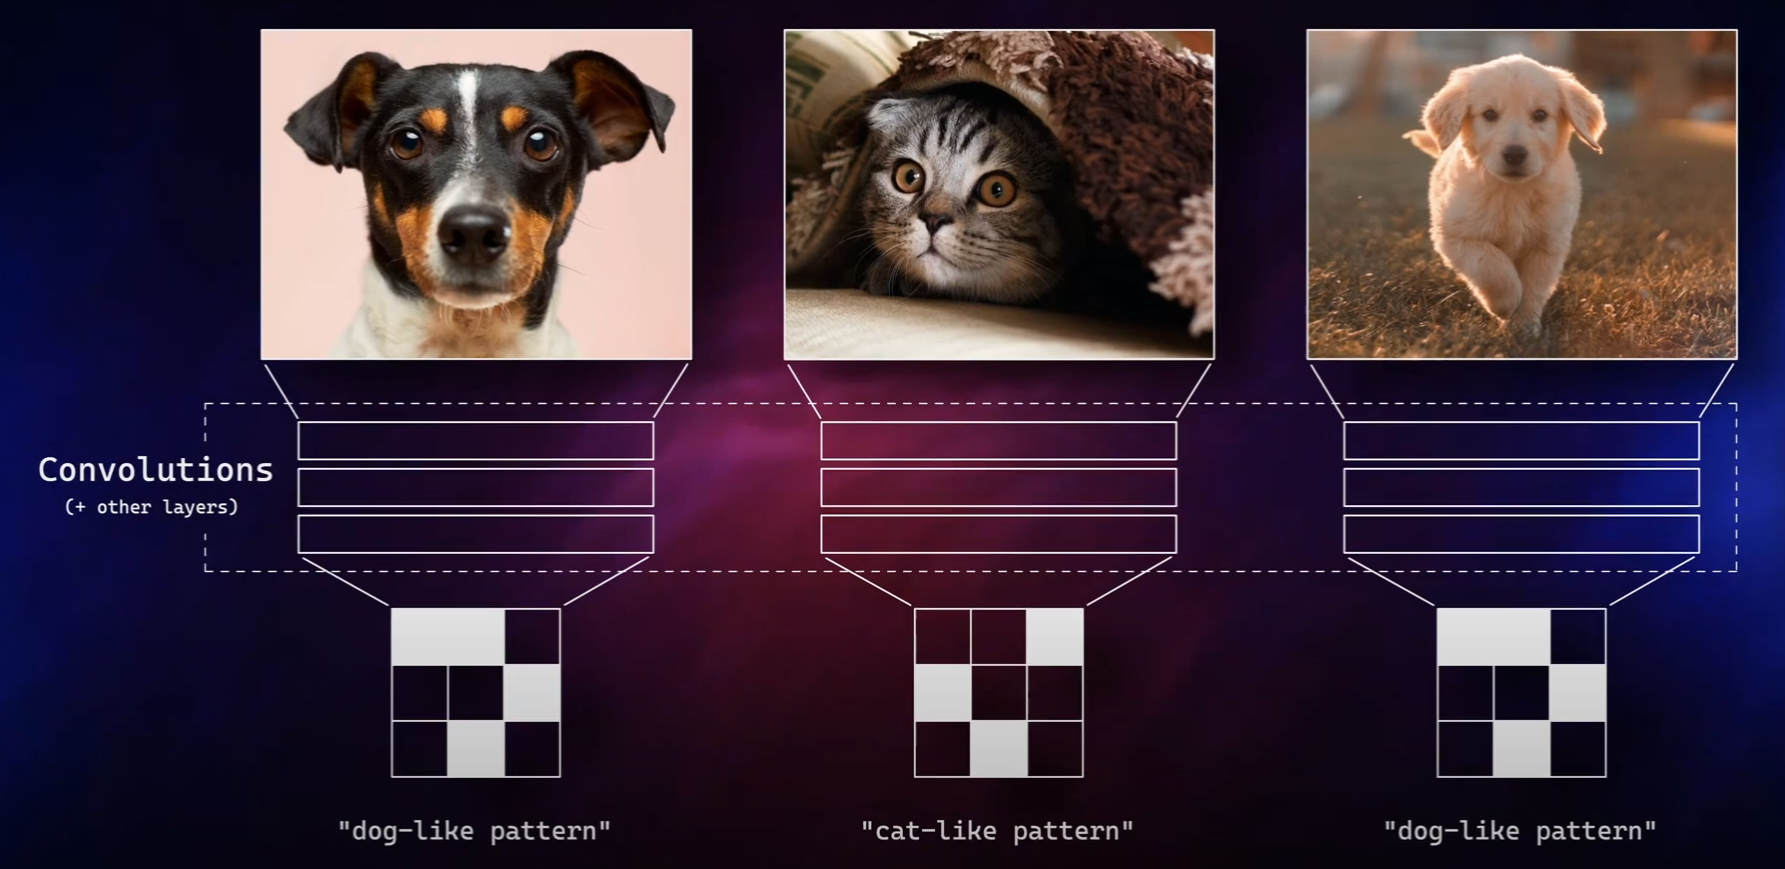
\includegraphics[width=0.8\textwidth,height=0.75\textheight,keepaspectratio]{images/cnn/what-makes-cnn.png}
    \end{figure}
\end{frame}

\begin{frame}{Components of a CNN}
    \begin{figure}
    \centering
    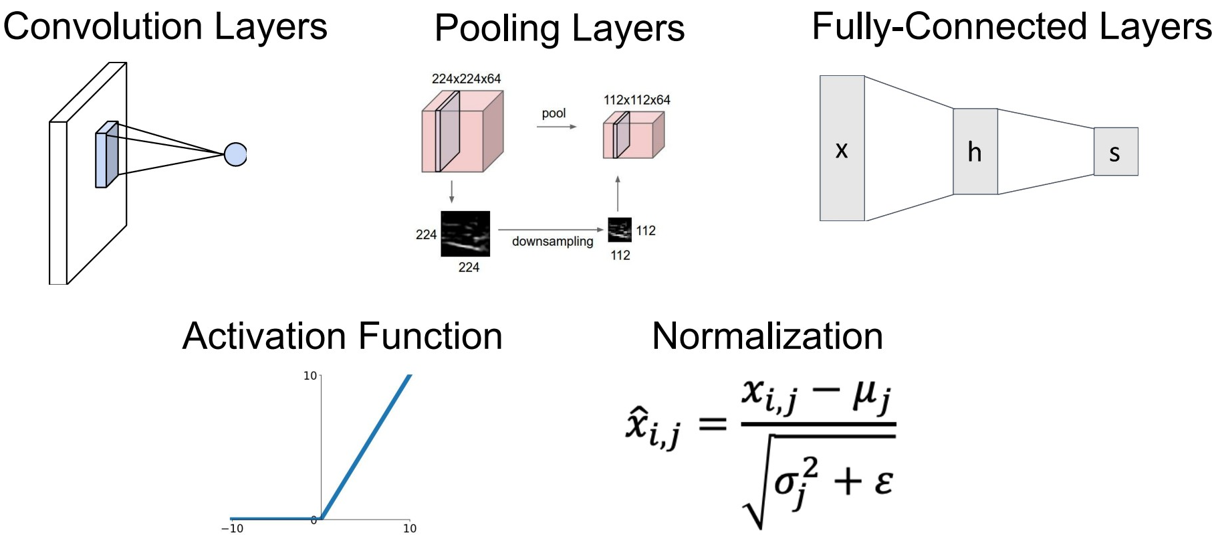
\includegraphics[width=0.95\textwidth,height=0.95\textheight,keepaspectratio]{images/cnn/cnn-components.png}
    \end{figure}
\end{frame}